%File: formatting-instructions-latex-2024.tex
%release 2024.0
\documentclass[letterpaper]{article} % DO NOT CHANGE THIS
\usepackage{aaai24}  % DO NOT CHANGE THIS
\usepackage{times}  % DO NOT CHANGE THIS
\usepackage{helvet}  % DO NOT CHANGE THIS
\usepackage{courier}  % DO NOT CHANGE THIS
\usepackage[hyphens]{url}  % DO NOT CHANGE THIS
\usepackage{graphicx} % DO NOT CHANGE THIS
\urlstyle{rm} % DO NOT CHANGE THIS
\def\UrlFont{\rm}  % DO NOT CHANGE THIS
\usepackage{natbib}  % DO NOT CHANGE THIS AND DO NOT ADD ANY OPTIONS TO IT
\usepackage{caption} % DO NOT CHANGE THIS AND DO NOT ADD ANY OPTIONS TO IT
\frenchspacing  % DO NOT CHANGE THIS
\setlength{\pdfpagewidth}{8.5in}  % DO NOT CHANGE THIS
\setlength{\pdfpageheight}{11in}  % DO NOT CHANGE THIS
%
% These are recommended to typeset algorithms but not required. See the subsubsection on algorithms. Remove them if you don't have algorithms in your paper.
\usepackage{algorithm}
\usepackage{algorithmic}

%
% These are are recommended to typeset listings but not required. See the subsubsection on listing. Remove this block if you don't have listings in your paper.
\usepackage{newfloat}
\usepackage{listings}
\DeclareCaptionStyle{ruled}{labelfont=normalfont,labelsep=colon,strut=off} % DO NOT CHANGE THIS
\lstset{%
	basicstyle={\footnotesize\ttfamily},% footnotesize acceptable for monospace
	numbers=left,numberstyle=\footnotesize,xleftmargin=2em,% show line numbers, remove this entire line if you don't want the numbers.
	aboveskip=0pt,belowskip=0pt,%
	showstringspaces=false,tabsize=2,breaklines=true}
\floatstyle{ruled}
\newfloat{listing}{tb}{lst}{}
\floatname{listing}{Listing}
%
% Keep the \pdfinfo as shown here. There's no need
% for you to add the /Title and /Author tags.
\pdfinfo{
/TemplateVersion (2024.1)
}

% DISALLOWED PACKAGES
% \usepackage{authblk} -- This package is specifically forbidden
% \usepackage{balance} -- This package is specifically forbidden
% \usepackage{color (if used in text)
% \usepackage{CJK} -- This package is specifically forbidden
% \usepackage{float} -- This package is specifically forbidden
% \usepackage{flushend} -- This package is specifically forbidden
% \usepackage{fontenc} -- This package is specifically forbidden
% \usepackage{fullpage} -- This package is specifically forbidden
% \usepackage{geometry} -- This package is specifically forbidden
% \usepackage{grffile} -- This package is specifically forbidden
% \usepackage{hyperref} -- This package is specifically forbidden
% \usepackage{navigator} -- This package is specifically forbidden
% (or any other package that embeds links such as navigator or hyperref)
% \indentfirst} -- This package is specifically forbidden
% \layout} -- This package is specifically forbidden
% \multicol} -- This package is specifically forbidden
% \nameref} -- This package is specifically forbidden
% \usepackage{savetrees} -- This package is specifically forbidden
% \usepackage{setspace} -- This package is specifically forbidden
% \usepackage{stfloats} -- This package is specifically forbidden
% \usepackage{tabu} -- This package is specifically forbidden
% \usepackage{titlesec} -- This package is specifically forbidden
% \usepackage{tocbibind} -- This package is specifically forbidden
% \usepackage{ulem} -- This package is specifically forbidden
% \usepackage{wrapfig} -- This package is specifically forbidden
% DISALLOWED COMMANDS
% \nocopyright -- Your paper will not be published if you use this command
% \addtolength -- This command may not be used
% \balance -- This command may not be used
% \baselinestretch -- Your paper will not be published if you use this command
% \clearpage -- No page breaks of any kind may be used for the final version of your paper
% \columnsep -- This command may not be used
% \newpage -- No page breaks of any kind may be used for the final version of your paper
% \pagebreak -- No page breaks of any kind may be used for the final version of your paperr
% \pagestyle -- This command may not be used
% \tiny -- This is not an acceptable font size.
% \vspace{- -- No negative value may be used in proximity of a caption, figure, table, section, subsection, subsubsection, or reference
% \vskip{- -- No negative value may be used to alter spacing above or below a caption, figure, table, section, subsection, subsubsection, or reference

\setcounter{secnumdepth}{0} %May be changed to 1 or 2 if section numbers are desired.

% The file aaai24.sty is the style file for AAAI Press
% proceedings, working notes, and technical reports.
%

% Title

% Your title must be in mixed case, not sentence case.
% That means all verbs (including short verbs like be, is, using,and go),
% nouns, adverbs, adjectives should be capitalized, including both words in hyphenated terms, while
% articles, conjunctions, and prepositions are lower case unless they
% directly follow a colon or long dash
\title{MapLE: Matching Molecular Analogues Promptly with Low\\ Computational Resources by Multi-Metrics Evaluation (Student Abstract)}
\author{
    %Authors
    % All authors must be in the same font size and format.
    Xiaojian Chen\textsuperscript{\rm 1, 2}, 
    Chuyue Liao\textsuperscript{\rm 1},
    Yanhui Gu\textsuperscript{\rm 1}, 
    Yafei Li\textsuperscript{\rm 3}, 
    Jinlan Wang\textsuperscript{\rm 4},  
    Yi Chen\textsuperscript{\rm 1},
    Masaru Kitsuregawa\textsuperscript{\rm 5}
}
\affiliations{
    %Afiliations
    
    % If you have multiple authors and multiple affiliations
    % use superscripts in text and roman font to identify them.
    % For example,

    % Sunil Issar\textsuperscript{\rm 2}, 
    % J. Scott Penberthy\textsuperscript{\rm 3}, 
    % George Ferguson\textsuperscript{\rm 4},
    % Hans Guesgen\textsuperscript{\rm 5}
    % Note that the comma should be placed after the superscript
    
    \textsuperscript{\rm 1}School of Computer and Electronic Information Science, Nanjing Normal University\\
    \textsuperscript{\rm 2}Department of Biomedical Engineering, Johns Hopkins University\\
    \textsuperscript{\rm 3}School of Chemistry and Materials Science, Nanjing Normal University\\
    \textsuperscript{\rm 4}School of Physics, Southeast University\\
    \textsuperscript{\rm 5}Institute of Industrial Science, The University of Tokyo\\
    % email address must be in roman text type, not monospace or sans serif
    \{xchen279, cliao, gu, liyafei\}@njnu.edu.cn, jlwang@seu.edu.cn, cs\_chenyi@njnu.edu.cn, kitsure@tkl.iis.u-tokyo.ac.jp

%
% See more examples next
}

%Example, Single Author, ->> remove \iffalse,\fi and place them surrounding AAAI title to use it
\iffalse
\title{My Publication Title --- Single Author}
\author {
    Author Name
}
\affiliations{
    Affiliation\\
    Affiliation Line 2\\
    name@example.com
}
\fi

\iffalse
%Example, Multiple Authors, ->> remove \iffalse,\fi and place them surrounding AAAI title to use it
\title{My Publication Title --- Multiple Authors}
\author {
    % Authors
    First Author Name\textsuperscript{\rm 1,\rm 2},
    Second Author Name\textsuperscript{\rm 2},
    Third Author Name\textsuperscript{\rm 1}
}
\affiliations {
    % Affiliations
    \textsuperscript{\rm 1}Affiliation 1\\
    \textsuperscript{\rm 2}Affiliation 2\\
    firstAuthor@affiliation1.com, secondAuthor@affilation2.com, thirdAuthor@affiliation1.com
}
\fi


% REMOVE THIS: bibentry
% This is only needed to show inline citations in the guidelines document. You should not need it and can safely delete it.
\usepackage{bibentry}
% END REMOVE bibentry

\begin{document}

\maketitle

\begin{abstract}
Matching molecular analogues is a computational chemistry and bioinformatics research issue which is used to identify molecules that are structurally or functionally similar to a target molecule. Recent studies on matching analogous molecules have predominantly concentrated on enhancing effectiveness, often sidelining computational efficiency, particularly in contexts of low computational resources. This oversight poses challenges in many real applications (e.g., drug discovery, catalyst generation and so forth). To tackle this issue, we propose a general strategy named \textbf{\textit{MapLE}}, aiming to promptly match analogous molecules with low computational resources by multi-metrics evaluation. Experimental evaluation conducted on a public biomolecular dataset validates the excellent and efficient performance of the proposed strategy.
\end{abstract}

\section{Introduction}
Matching analogues involves the identification of molecules that resemble original compounds based on their chemical, pharmacological, and structural characteristics. When applied to drug discovery, this procedure is of paramount importance, as it could considerably hasten the investigation of potential therapeutic agents. Indeed, there are numerous untapped opportunities for drug discovery originating from natural products~\cite{DeCorte2016}.

Most recent studies on matching analogues have primarily focused on improving similarity screening accuracy rather than on time efficiency optimization~\cite{Chen2023}. Nonetheless, current methodologies tend to slow down when employed with fully enumerated chemical libraries, which may contain billions of compounds.They often become impractical due to the substantial computational resources required~\cite{Sadybekov2023}.
Warr et al. introduced Arthor, utilizing the RoundTable algorithm, which could search for patterns over a billion molecules in a few seconds~\cite{Warr2022}. However, search time scales with database size, and the vast growth of chemical space may pose challenges.

To address these challenges, we introduce a general framework that incorporates several efficient strategies. Specifically, we perform multiple feature extraction on processed molecular objects and a progressive evaluation strategy to match the analogs promptly. 
By integrating data from these multiple features, our framework results in competitive evaluation performance and a better understanding of the impact of various information sources. 
In addition, we streamline the molecule accesses in the process of molecule matching by a progressive prompt evaluation, ultimately reducing the execution time and computational resources.

\section{Proposed Strategy}
% \begin{figure*}[t]
% 	\centering % avoid the use of \begin{center}...\end{center} and use \centering instead (more compact)
% 	\includegraphics[width=\linewidth]{images/framework7.eps}
% 	\caption{
% 		The general framework of \textbf{\textit{MapLE}}.
% 	}
% 	\label{figure:framwork}
% \end{figure*} 

\begin{figure*}[htp]
	\centering % avoid the use of \begin{center}...\end{center} and use \centering instead (more compact)
	\includegraphics[width=\linewidth  ]{images/framework10.eps}
	\caption{
		The general framework of \textbf{\textit{MapLE}}. 
	}
	\label{figure:framwork}
\end{figure*}

As shown in Figure~\ref{figure:framwork}, we introduce \textbf{\textit{MapLE}}---a general  framework for \textbf{M}atching molecular \textbf{a}nalogues \textbf{p}romptly with \textbf{L}ow
computational resources by multi-metrics \textbf{E}valuation---which integrates multiple similarity metrics and introduces a progressive prompt evaluation technique tailored to speed up the screening process.

\subsubsection{Multi-metrics Fusion.}
Our approach intuitively considers multiple attributes of a molecule and synthesize them into a cohesive evaluation. As depicted in Figure~\ref{figure:framwork} (a), our general framework is hierarchical, incorporating various features of the molecule. Specifically, we rank the similarity among molecules within a set by considering pharmacological, structural, and chemical features in a multi-metrics evaluation. Moreover, within the category of structural features, we further employ sub-metrics (e.g., $topo1$, $topo2$, and $topo3$) to analyze the molecule from multiple topological perspectives~\cite{Kim2023}.

To efficiently manage these features, we construct a set of inverted lists. It is important to note that each new molecule is broken down into several feature indices. When adding a new molecule to the database, we only need to update the lists containing these specific indices. Thereby, this approach minimizes irrelevant traversal queries, thus saving time, especially when dealing with large databases.


\subsubsection{Progressive Prompt Evaluation.}
Inspired by the search for the top-\textit{k} semantically similar sentences in the field of Natural Language Processing (NLP), we build a mapping between molecular structures and word sentences. 
Specifically, we consider the substructures or features of a molecule analogous to the words in sentences.
We outline our strategy for measuring the similarity between query molecules $Q$ and the top-\textit{k} candidate similar molecule $L$, as follows:
\begin{equation}
    \widetilde{Sim}_{metric}(L, Q) = \frac{\sum\limits_{i=1}^\delta(f_{L}(i) \wedge f_{Q}(i))}{\sum\limits_{i=1}^\delta(f_{L}(i)\vee f_{Q}(i))}
\end{equation}
where $f(i)$ is the frequency of the \textit{i}-th feature in the molecule, $\delta$ is the size of the whole molecular features, and we use the tanimoto coefficient to compute similarity under a single metric of $L$ and $Q$ as $Sim_{metric}(L, Q)$. To consolidate these different metrics of similarity, we present the similarity as:
\begin{equation}
    \widetilde{Sim}(L, Q) = \sum w_{j} \cdot \widetilde{Sim}_{j}(L, Q)
\end{equation}
where $\widetilde{Sim}_{j}$ is measured under a specific metric similarity, and $w_j$ denotes the corresponding weight of the metric.

We propose an efficient strategy to assemble the on-the-fly. We denote that $\widetilde{Sim_j}^{top-k}$ is the normalized similarity score of the top-\textit{k} molecule in the metric $j$, and the $t$ is the threshold where $t = \sum w_j \cdot \widetilde{Sim_j}^{top-k}$. We will progressively output the top-\textit{k} result when a candidate molecule $L$ meet the condition that $\widetilde{Sim}(L, Q) \geq t$, since it is at least for one metric that $\widetilde{Sim_j}(P, Q) \geq \widetilde{Sim_j}^{top-k}$. It means we only matching the top of molecule list rather than traversal the whole list, which will save a lot query time to get top-\textit{k} analogues.
More details shown in Figure~\ref{figure:framwork} (b) make a example of our strategy.


\section{Experiments}
\begin{figure}[htp]
	\centering % avoid the use of \begin{center}...\end{center} and use \centering instead (more compact)
	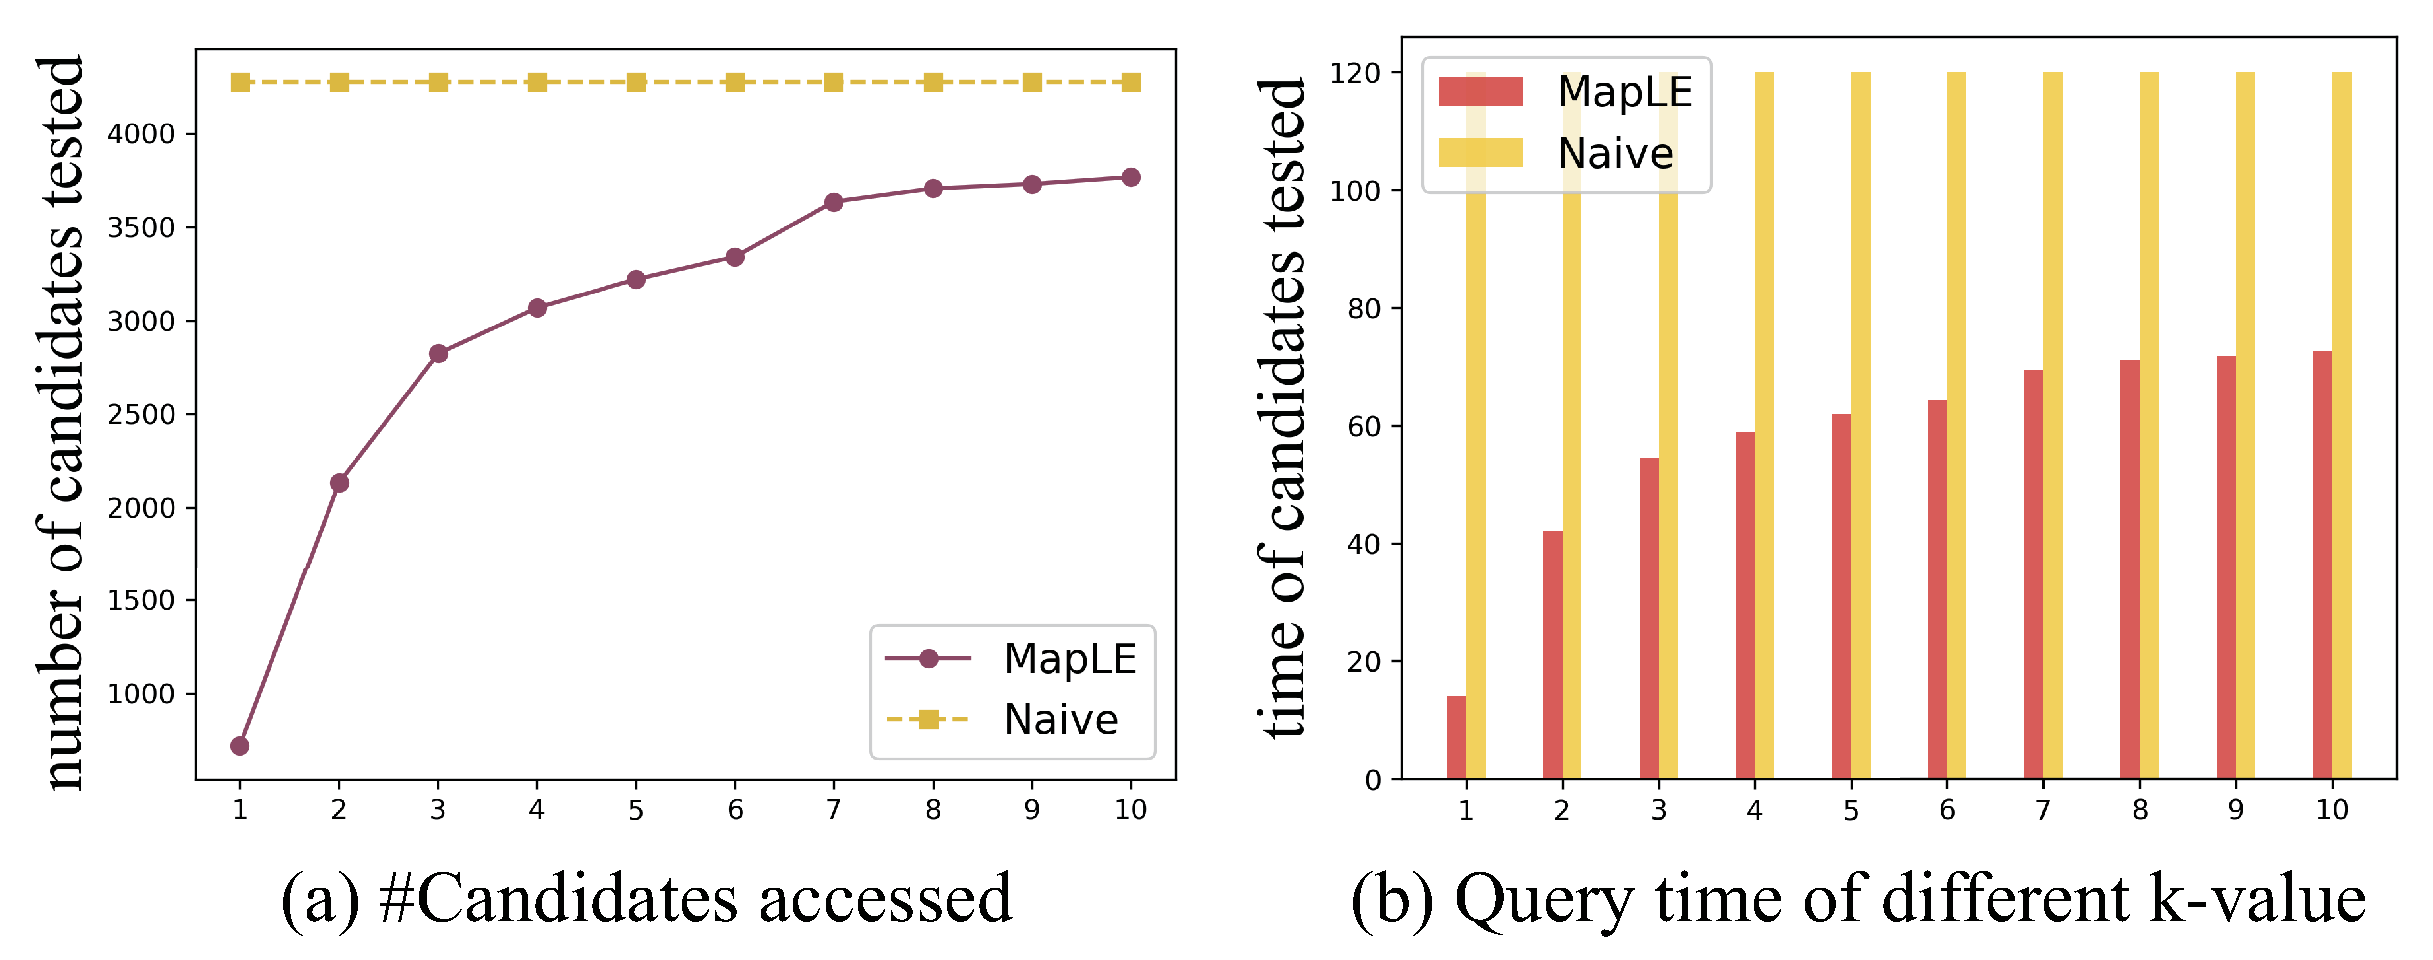
\includegraphics[width=\linewidth  ]{images/result_cost2.eps}
	\caption{
		The evaluation result of the \textbf{\textit{MapLE}}.
	}
	\label{figure:result_cost}
\end{figure}
We conducted our experiments on the CASF-2016 dataset, a widely-used biomolecular dataset with thousands of high-quality molecular structures. As shown in Figure \ref{figure:result_cost} (a), the baseline accesses all the ligand molecules in the dataset, with the query time remaining consistent regardless of the value of $k$. Notably, the top-1 values are returned almost instantly, and as $k$ increases, a progressively greater number of results are obtained. In comparison, our proposed method showcases its efficiency, particularly with smaller values of $k$. Additionally, we monitored the number of accessed candidate values. Figure \ref{figure:result_cost} (b) details the count of candidates accessed during the data collection phase.
% \section{Conclusion}
% In this paper, we introduce a general framework for matching molecular analogues based on multi-metrics evaluation. This framework incorporates several strategies that are both time-efficient and computational resource-saving. Our experimental evaluation, conducted on a real bio-molecular dataset, attests to the framework's effectiveness. In the future, we aim to validate the performance of various metrics and assess their impact on the results, thereby enhancing the interpretability of the framework.

\section{Acknowledgments}
This work is supported by National Natural Science Foundation of China (Grant No.92370127 and No.22033002).

\bibliography{aaai24}

\end{document}
